\chapter{Redes de interacción entre tortugas}
\graphicspath{{figs/}}

\chapterquote{In retrospect, Euler's unintended message is very simple: Graphs or networks have properties, hidden in their construction, that limit or enhance our ability to do things with them.}{Albert-László Barabási, 1982}

\label{Redes de interacción entre tortugas}
\section{Trayectorias }

Primero se muestran las trayectorias obtenidas para un día de medición (Fig.~\ref{fig:trayeSinFiltr}), como por ejemplo 1/12/2020. Para éstas se realizó un programa en el lenguaje Python utilizando la librería Folium, permitiendo añadir puntos de GPS al mapa \cite{github}.
 
\begin{figure}[h]
    \begin{center}
       
   
    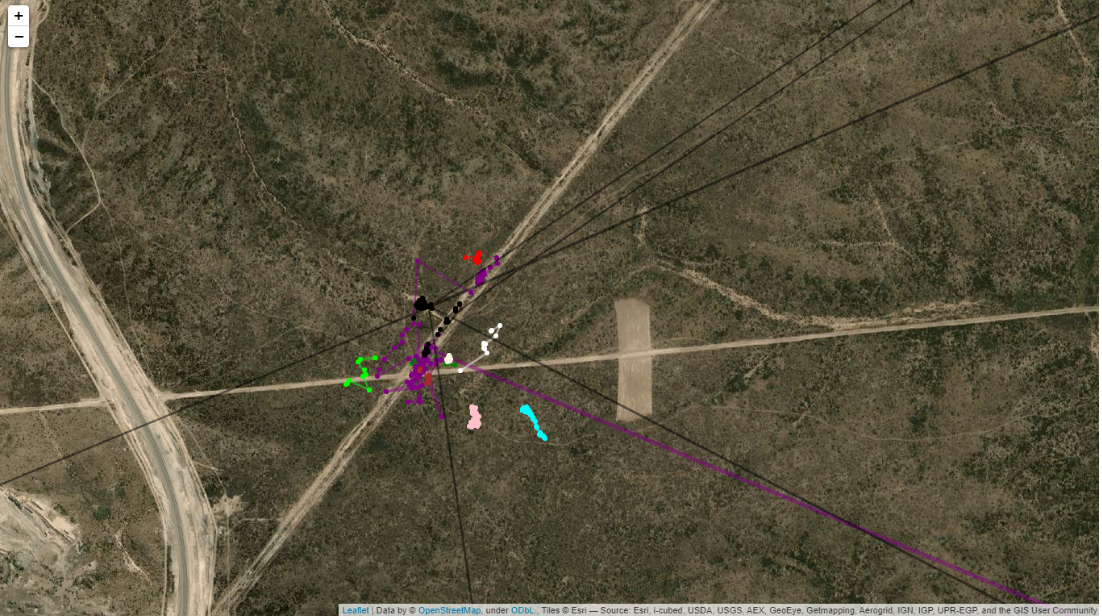
\includegraphics[width=.9\textwidth]{Chap2/Traye1_12_sinF.png}
\end{center}
    \caption[Trayectorias un dia de medición, sin filtrrar.]{Trayectorias del 1/12/2020, cada color representa una tortuga diferente. Ambas metodologías fueron implementadas, algunos puntos tomados con el tortugómetro escapan a la trayectoria esperada.}
    \label{fig:trayeSinFiltr}
\end{figure}
Se observa en la Fig.~\ref{fig:trayeSinFiltr}, que algunos puntos tomados por el tortugómetro se desvían de la trayectoria esperada para una tortuga (recorren distancias del orden de los kilómetros en menos de 10 minutos). Se estima que estas desviaciones se producen por dos motivos: en primer lugar, en los primeros minutos de medición, el GPS comienza a conectarse a satélites hasta tener la precisión máxima, haciendo que  los primeros puntos tengan una mayor desviación; en segundo lugar, se observó de manera aleatoria la desviación de algún punto respecto de la trayectoria típica.
 
 
 
 
Para corregir estas desviaciones, se implementó un método basado en la velocidad máxima que pueden alcanzar los individuos. El mismo está detallado en el repositorio de GitHub, archivo \textit{CriterioParaSacarData.py} \cite{github}. Para obtener la velocidad máxima, se calculó la distribución de velocidades de la Fig.~\ref{fig:distribuciondeVel}.

 
Se observó en la distribución de velocidades de la Fig.~\ref{fig:distribuciondeVel}, que las tortugas llegan a una velocidad máxima de aproximadamente 15m/min, de manera que se adoptó el criterio de filtrar los tramos de trayectoria en los que la velocidad supera ese valor máximo. Filtrando los puntos de la Fig.~\ref{fig:trayeSinFiltr}, tomando velocidad máxima 15 m/min, se obtuvo  el mapa de la Fig.~\ref{fig:trayeConFiltr}.
 
 
\begin{figure}[h]
\begin{center}
       
   
    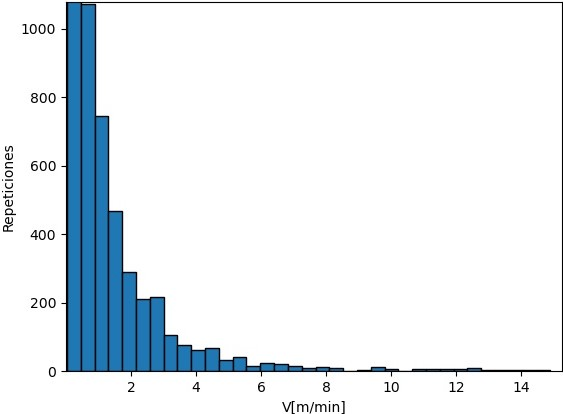
\includegraphics[width=.7\textwidth]{Chap2/Velocidades2.jpeg}
    \caption[Distribución de velocidades.]{Histograma de velocidades en m/min. Las  velocidades obtenidas mayores a 15 m/min están órdenes de magnitud por encima.}
    \label{fig:distribuciondeVel}
\end{center}
\end{figure}
 

\begin{figure}[h]
    \begin{center}
       
   
    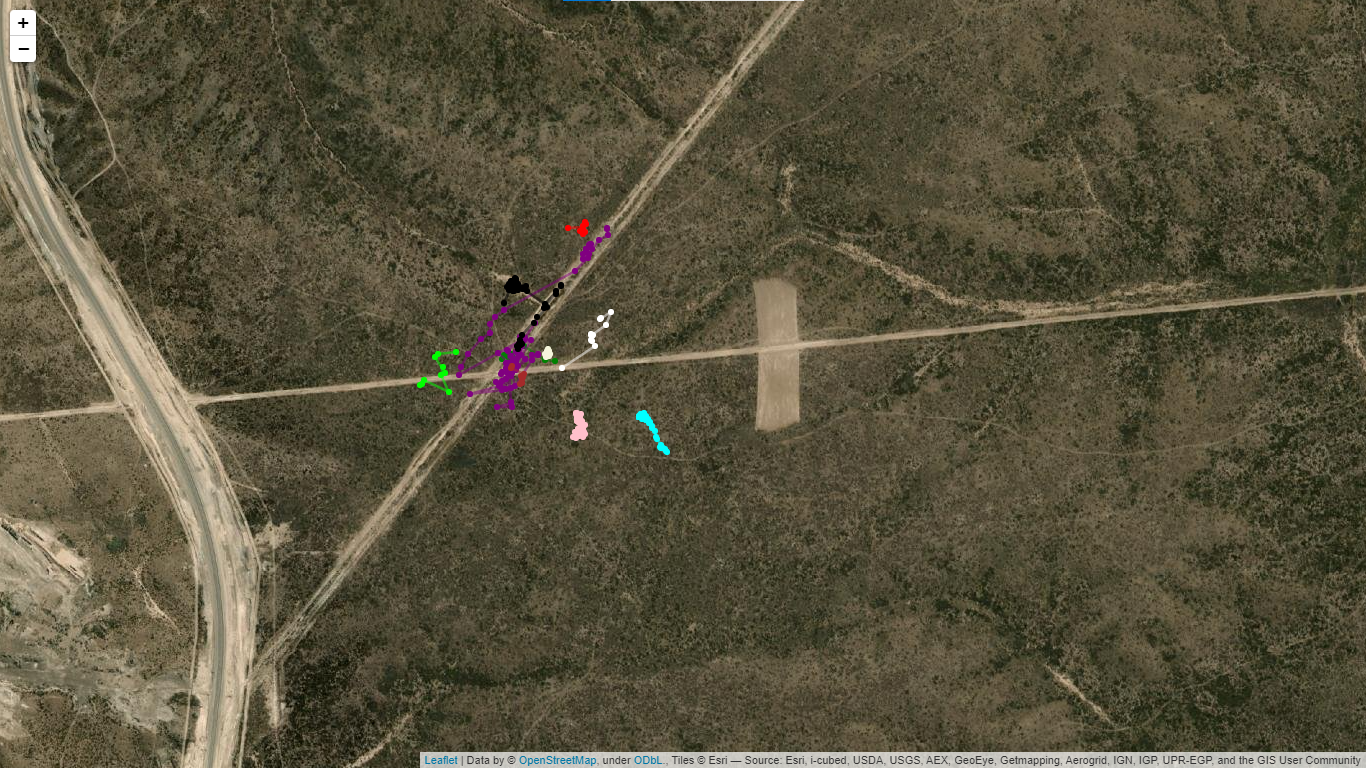
\includegraphics[width=.9\textwidth]{Chap2/Traye1_12_conF.png}
\end{center}
    \caption[Trayectorias un dia de medición, despues del filtrado.]{Trayectorias del 1/12/2020 luego del filtrado, cada color representa una tortuga diferente.}
    \label{fig:trayeConFiltr}
\end{figure}
\begin{Huge}
Idea : conectar con criterio de encuentros mostrar grafico de encuentros segun la epoca del año y pasar a las dos redes de interacción que tenemos 
\end{Huge}

%%% Local Variables: 
%%% mode: latex
%%% TeX-master: "template"
%%% End: 
